\documentclass[a4paper, 12pt]{article}
\usepackage[margin=1in]{geometry}
\usepackage[english]{babel}
\usepackage[utf8]{inputenc}
\usepackage{amsmath}
\usepackage{mathtools}
\usepackage{color, soul}
\usepackage{xcolor}
\usepackage{tcolorbox}
\usepackage{listings}
\usepackage{graphicx}
\usepackage{textcomp}
\usepackage{url}
\tcbuselibrary{breakable}

%% MATLAB
\definecolor{codegreen}{rgb}{0,0.6,0}
\definecolor{codegray}{rgb}{0.5,0.5,0.5}
\definecolor{codepurple}{rgb}{0.58,0,0.82}
\definecolor{backcolour}{rgb}{0.95,0.95,0.92}

\lstdefinestyle{mystyle}{
	backgroundcolor = \color{backcolour},
	commentstyle = \color{codegreen},
	keywordstyle = \color{magenta},
	numberstyle = \tiny\color{codegray},
	stringstyle=\color{codepurple},
	basicstyle=\ttfamily\footnotesize,
	breakatwhitespace=false,
	breaklines=true,
	captionpos = b,
	keepspaces = true,
	numbers = left,
	numbersep = 5pt,
	showspaces = false,
	showstringspaces = false,
	showtabs = false,
	tabsize = 2
}

\lstset{style=mystyle}

%%%

\begin{document}
\title{BRI509: Introduction to Brain Signal Processing \\ Assignment No. 1}
\author{\underline{\textbf{CANOY RAYMART JAY}} \\ 
Student ID \#: \underline{\textbf{2020021376}}}
\date{\today}
\maketitle


\begin{itemize}
\item[\textbf{1.}]{\textbf{Explain the following terms briefly.}}
\begin{itemize}
\item[\textbf{(a)}]{\textbf{Sampling property of the impulse}}

\begin{tcolorbox}
The sampling property is one of the important properties of the unit impulse which follows the equivalence property. According to the equivalence property, the product of an arbitrary function $g(t)$ and the unit impulse $\delta (t - t_{0})$ can be written as:
\begin{equation}
g(t)\delta(t - t_{0}) = g(t_{0})\delta(t - t_{0}).
\end{equation}
Hence,
\begin{equation}
\begin{gathered}
\begin{alignedat}{1}
\int_{-\infty}^{\infty}{g(t)\delta(t - t_{0})dt} &= \int_{-\infty}^{\infty}{g(t_{0})\delta(t - t_{0})dt}, \\
&= g(t_{0})\int_{-\infty}^{\infty}{\delta(t - t_{0})dt} \\
&= g(t_{0})
\end{alignedat}
\end{gathered}
\end{equation}
The sampling property of the impulse, therefore, means that in an integral of this type, the impulse will sample the value of the arbitrary function $g(t)$ at time $t = t_{0}$. 
\end{tcolorbox}

\item[\textbf{(b)}]{\textbf{Time invariance}}

\begin{tcolorbox}
Time invariance is one of the system properties wherein a time-shifted input signal will also cause a time-shifted response. Mathematically, if a system is initially in its zero state and an arbitrary input signal $x(t)$ causes a response $y(t)$, then a time-shifted input signal $x(t - t_{0})$ will also cause a time-shifted response $y(t-t_{0})$ for any arbitrary $t_{0}$.
\end{tcolorbox}

\pagebreak

\item[\textbf{(c)}]{\textbf{Causality}}

\begin{tcolorbox}
Causality is one of the system properties wherein a system responds only during or after the time in which it is excited. It is important to take note that all physical systems are causal because they cannot look into the future and respond before they are being excited.
\end{tcolorbox}
\item[\textbf{(d)}]{\textbf{Linearity and Superposition}}

\begin{tcolorbox}
\textcolor{red}{\textbf{Linearity}} is a property of homogeneous and additive systems. It is important to take note that:
\begin{itemize}
\item{In a homogeneous system, if the input signal is multiplied by a constant (including complex constants), then the zero-state response is also multiplied by the same constant.}
\item{On the other hand, in an additive system, if the input signal $x_{1}(t)$ produces a zero-state response $y_{1}(t)$ and $x_{2}(t)$ produces $y_{2}(t)$, then the sum of the two input signals $x_{1}(t)$ and $x_{2}(t)$ will also produce a zero-state response which is the sum of the zero-state responses $y_{1}(t)$ and $y_{2}(t)$.}
\end{itemize}

Since linearity is a combination of these two properties, then  a linear system has these characteristics:
\begin{equation}
\begin{gathered}
\begin{alignedat}{1}
x_{1}(t) &\xrightarrow{\text{produces \; a \; zero-state \; response}} y_{1}(t), \\
x_{2}(t) &\xrightarrow{\text{produces \; a \; zero-state \; response}} y_{2}(t), \\
\left( \alpha x_{1}(t) + \beta x_{2}(t) \right)&\xrightarrow{\text{produces \; a \; zero-state \; response}} \left( \alpha y_{1}(t) + \beta y_{2}(t) \right).
\end{alignedat}
\end{gathered}
\end{equation}

\textcolor{red}{\textbf{Superposition}}, on the other hand, is a consequence of linearity wherein when one input signal is added to another, then the overall response is one of the responses added to the other as well. This implies that in a linear system, the zero-state response to a complicated input signal can be found by breaking the input signal down into simple pieces that add up to the original signal, finding the response to each small piece, and then adding all those responses to find the overall response to the overall complicated input signal.
\end{tcolorbox}

\item[\textbf{(e)}]{\textbf{Zero-input response vs. Zero-state response}}

\begin{tcolorbox}
If the input signal is $x(t)$, then the zero-input response is the solution to the differential or difference equation, which describes the dynamics of the system, when \underline{$x(t)$ is set to zero}. This is also called the homogeneous solution.\\

Zero-output response, on the other hand, is the solution to the differential or difference equation when the system has no stored energy, i.e., when the initial conditions are set to zero.
\end{tcolorbox}
\end{itemize}
\end{itemize}

\begin{itemize}
\item[\textbf{2.}]{\textbf{Solve the following simple problems.}}
\begin{itemize}
\item[\textbf{(a)}]{\textbf{What is the fundamental period of $g(t) = 2 \cos \left( 300 \pi t \right)$?}}\\
\textbf{\textcolor{red}{\textbf{Solution:}}}
\begin{enumerate}
\item[(i)]{Note that}
\begin{equation}
g(t) = A \cos \left(2 \pi f_{0}t \right) = 2\cos \left(300 \pi t \right).
\label{eq:prob2a}
\end{equation}
\item[(ii)]{By equating the arguments of the sinusoidal functions in eq. \eqref{eq:prob2a}, the fundamental frequency can be easily solved and can be written as:}
\begin{equation}
\begin{gathered}
\begin{alignedat}{1}
2 \pi f_{0} t & = 300 \pi t, \\
f_{0} & = \frac{300 \pi t}{2 \pi t}, \\
f_{0} & = 150 \; \; \mathtt{cycles/s}.
\end{alignedat}
\end{gathered}
\end{equation}
\item[(iii)]{Therefore, the fundamental period is}
\begin{equation}
\begin{gathered}
\begin{alignedat}{1}
T_{0} &= \frac{1}{f_{0}}, \\
\Aboxed{T_{0} &= \frac{1}{150} \; \; \mathtt{s}.}
\end{alignedat}
\end{gathered}
\end{equation}
\end{enumerate}

\item[\textbf{(b)}]{\textbf{Find and graph the even parts of the function $g(t)$}}
\begin{figure}[h!]
\center{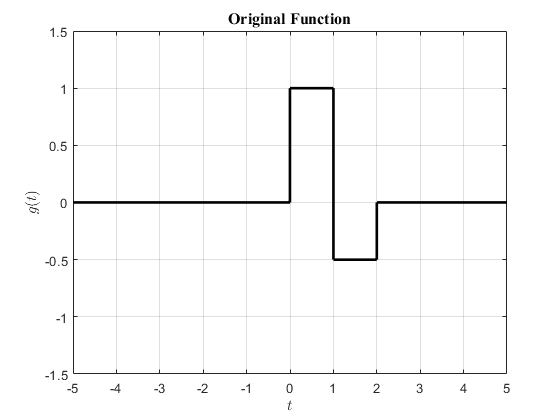
\includegraphics[width=12cm]{prob2b_originalFunction.png}}
\caption{\label{fig:2b_originalFunction} The original function $g(t)$.}
\end{figure}

\textcolor{red}{\textbf{Solution:}}
\begin{itemize}
\item[(i)]{This function can be represented mathematically as:}
\[
\boxed{
g(t) =
\begin{cases}
0, & t < 0 \\
1, & 0 \leq t \leq 1 \\
-\frac{1}{2}, & 1 < t \leq 2 \\
0, & t > 2
\end{cases}
}
\]
\item[(ii)]{The even and odd parts  of the function $g(t)$ can be written as}
\begin{equation}
g_{e}(t) = \frac{g(t) + g(-t)}{2}, \; \; \; \mathtt{and} \; \; \; g_{o}(t) = \frac{g(t) - g(-t)}{2},
\end{equation}
respectively, where $g(-t)$ is the time-reversed function of $g(t)$. This time-reversed function can be represented mathematically as:
\[
\boxed{
g(-t) = 
\begin{cases}
0, & t > 0 \\
1, & -1 \leq t \leq 0 \\
-\frac{1}{2}, & -2 \leq t < -1 \\
0, & t < -2
\end{cases}
}
\]
\begin{figure}[h!]
\center{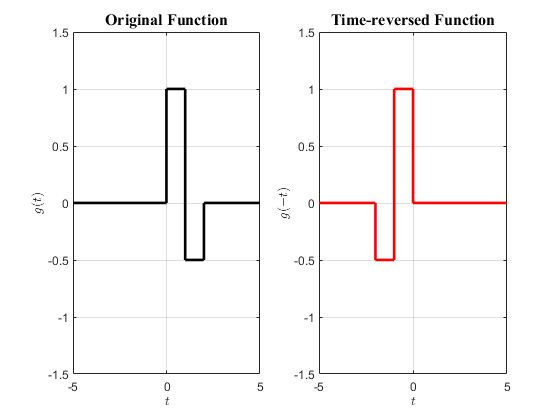
\includegraphics[width=12cm]{prob2b_Fig2_timeReversed.png}}
\caption{\label{fig:2bFig2}The graphs of the original function $g(t)$ and the time-reversed function $g(-t)$.}
\end{figure}
\item[(iii)]{The even part, $g_{e}(t)$,  of the function $g(t)$, therefore, can be calculated as}
\begin{equation}
\begin{gathered}
\begin{alignedat}{1}
g_{e}(t) &= \frac{g(t) + g(-t)}{2} \\
g_{e}(t) &= \frac{1}{2}
\begin{cases}
0, & t < -2 \\
-\frac{1}{2}, & -2 \leq t < -1 \\
1, & -1 \leq t < 0 \\
2, & t = 0 \\
1, & 0 < \leq 1 \\
-\frac{1}{2}, & 1 < t \leq 2 \\
0, & t > 2
\end{cases} \\
g_{e}(t) &=
\begin{cases}
0, & t < -2 \\
-\frac{1}{4}, & -2 \leq t < -1 \\
\frac{1}{2}, & -1 \leq t < 0 \\
1, & t = 0 \\
\frac{1}{2}, & 0 < \leq 1 \\
-\frac{1}{4}, & 1 < t \leq 2 \\
0, & t > 2 
\end{cases}
\end{alignedat}
\end{gathered}
\end{equation}
\begin{figure}[h!]
\center{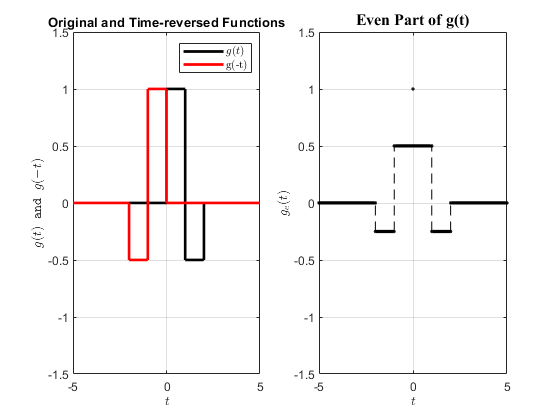
\includegraphics[width=12cm]{prob2b_Fig3_evenPart.png}}
\caption{The graphs of the original function $g(t)$, time-reversed function $g(-t)$, and the \textcolor{red}{\textbf{even part}}, $g_{e}(t)$, of the of the function $g(t)$.}
\end{figure}
\item[(iv)]{The odd part, $g_{o}(t)$, of the function $g(t)$ can, therefore, be calculated as:}
\begin{equation}
\begin{gathered}
\begin{alignedat}{1}
g_{o}(t) & = \frac{g(t) - g(-t)}{2} \\
g_{o}(t) & = \frac{1}{2}
\begin{cases}
0, & t < -2 \\
0- \left( - \frac{1}{2} \right), & -2 \leq t < -1 \\
0 - 1, & -1 < t < 0 \\
1 - 1, & t = 0 \\
1 - 0, & 0 \leq t < 1 \\
-\frac{1}{2} - 0, & 1 < t \leq 2 \\
0, & t > 2
\end{cases} \\
g_{}(t) & = 
\begin{cases}
0, & t < -2 \\
\frac{1}{4}, & -2 \leq t < -1 \\
- \frac{1}{2}, & -1 < t < 0 \\
0, & t = 0 \\
\frac{1}{2} , & 0 \leq t < 1 \\
-\frac{1}{4}, & 1 < t \leq 2 \\
0, & t > 2
\end{cases}
\end{alignedat} 
\end{gathered}
\end{equation}
\begin{figure}[h!]
\center{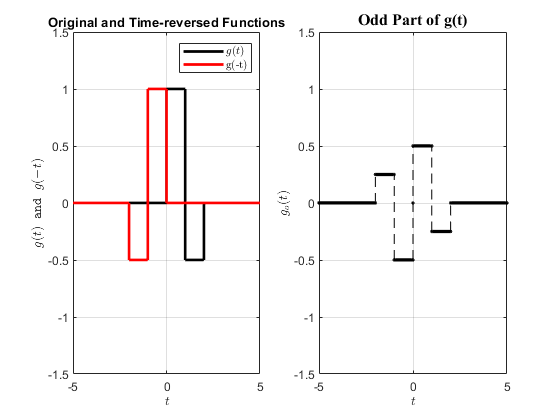
\includegraphics[width=12cm]{prob2b_Fig4_oddPart.png}}
\caption{The graphs of the original function $g(t)$, time-reversed function $g(-t)$, and the \textcolor{red}{\textbf{odd part}}, $g_{0}(t)$, of the of the function $g(t)$.}
\end{figure}
\end{itemize}

\pagebreak
\item[\textbf{(c)}]{\textbf{What is the numerical value of the following accumulation?}}
\begin{equation}
\sum_{n = -5}^{10} \delta_{3}[n]
\end{equation}
\textcolor{red}{\textbf{Solution:}}
\begin{itemize}
\item[(i)]{Note that impulse train is represented as $\delta_{N} = \sum_{m = -\infty}^{\infty}\delta[n - mN]$. If $N = 3$, the impulse train becomes $\boxed{\delta_{3}[n] = \sum_{m = -\infty}^{\infty}\delta[n - m(3)]}$. In the domain $-5 \leq n \leq 10$, this impulse train can be plotted as:}
\begin{figure}[h!]
\center{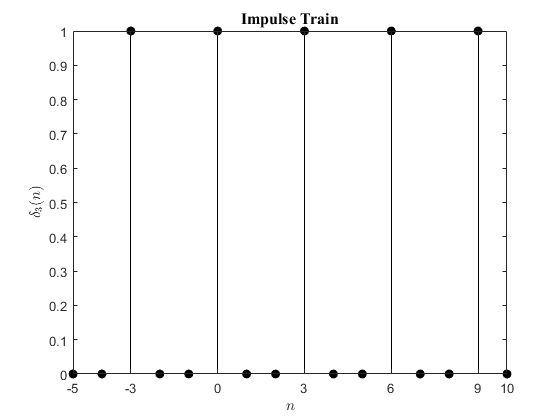
\includegraphics[width=8cm]{prob2c_Fig1_impulseTrain.png}}
\caption{\label{fig:prob2c_impulseTrain} The plot of the impulse train $\delta_{3}[n] = \sum_{m=-\infty}^{\infty}{\delta[n - m(3)]}$.}
\end{figure}
\item[(ii)]{The numerical value of the accumulation is shown in Fig. \eqref{fig:prob2c_accumulation}. It should be noted that it is assumed that the accumulation before $n = -5$ is zero.}
\begin{figure}[h!]
\center{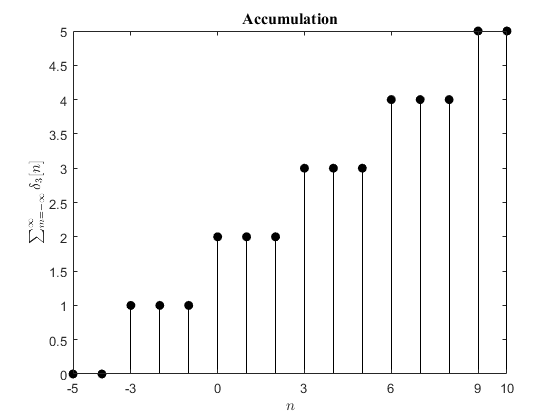
\includegraphics[width=8cm]{prob2c_Fig2_Accumulation.png}}
\caption{\label{fig:prob2c_accumulation}The accumulation of the impulse train $\delta_{3}[n]$}
\end{figure}
\end{itemize}

\pagebreak
\item[\textbf{(d)}]{\textbf{Find the average signal power of the periodic signal $x(t)$.}}
\begin{equation}
x(t) = A \cos \left(2 \pi f t \right)
\end{equation}
\textcolor{red}{\textbf{Solution:}}
\begin{equation}
\begin{gathered}
\begin{alignedat}{1}
P_{x}(t) & = \lim_{T \to \infty} \frac{1}{T} \int_{-T/2}^{T/2}{|x(t)|^{2}dt} \\
 & = \frac{1}{T_{0}} \int_{-T_{0}/2}^{T_{0}/2}{|A\cos \left(2 \pi f_{0} t \right)|^{2}dt} \\
 & = \frac{2|A|^{2}}{T_{0}} \int_{0}^{T_{0}/2}{\cos^{2} \left( 2 \pi f_{0} t\right) dt}
\end{alignedat}
\end{gathered}
\end{equation}
Note that $\cos (2A) = 2\cos^{2}(A) - 1$. Therefore, $\cos^{2}(A) = \frac{1}{2} \left(\cos(2A) + 1 \right)$.
\begin{equation}
\begin{gathered}
\begin{alignedat}{1}
P_{x}(t) &= \frac{2|A|^{2}}{T_{0}}\int_{0}^{T_{0}/2}{\frac{1}{2}\left(\cos(4\pi f_{0} t) + 1 \right) dt} \\
& = \frac{|A|^{2}}{T_{0}} \left[ \int_{0}^{T_{0}/2}{\cos(4\pi f_{0} t) dt } + \int_{0}^{T_{0}/2}{dt} \right] \\
&= \frac{|A|^{2}}{T_{0}} \left[ \frac{1}{4 \pi f_{0}}\Biggr( \sin\left(4 \pi f_{0} t \right) \Biggr\rvert_{0}^{T_{0}/2} + \frac{T_{0}}{2} \right] \\
& = \frac{|A|^{2}}{T_{0}} \left[ \frac{1}{4\pi f_{0}} \left( \sin(2\pi) - \sin(0)\right)  + \frac{T_{0}}{2}\right] \\
&= \frac{|A|^{2}}{T_{0}}\left( \frac{T_{0}}{2}\right) \\
\Aboxed{P_{x} &= \frac{|A|^{2}}{2}}
\end{alignedat}
\end{gathered}
\end{equation}

\pagebreak
\item[\textbf{(e)}]{\textbf{Graph the following function:}}
\begin{equation}
g[n] = 5 u[n - 1] - u [4 - n]
\end{equation}
\textcolor{red}{\textbf{Solution:}}
\begin{figure}[h!]
\center{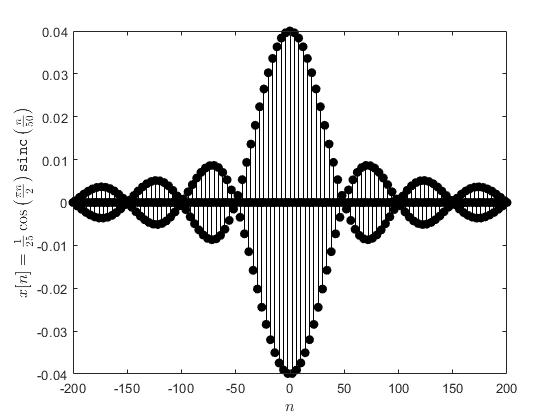
\includegraphics[width=18cm]{prob2e.png}}
\end{figure}
\end{itemize}
\end{itemize}

\pagebreak
\begin{itemize}
\item[\textbf{3.}]{\textbf{Solve the following problems}}
\begin{itemize}
\item[\textbf{(a)}]{\textbf{Find the zero-input response, the response when $x(t) = 0$, of the system in the figure if the initial value of $y(t)$ is $y(0) = 1$, and the initial rate of change of $y(t)$ is $y^{'}(t = 0) = 0$, $a = 1$, $b = 0$, and $c=4$.}}
\begin{figure}[h!]
\center{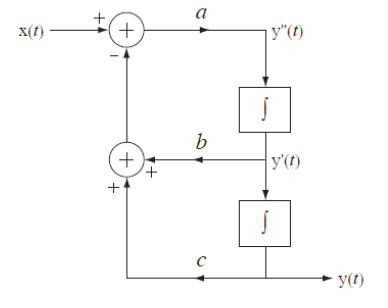
\includegraphics[width=8cm]{prob3a_probFig.png}}
\end{figure} \\
\textcolor{red}{\textbf{Solution:}}
\begin{itemize}
\item[(i)]{The differential equation which represents this system can be written as:}
\begin{equation}
\begin{gathered}
\begin{alignedat}{1}
y^{''}(t) &= a \left[ x(t) - \left(b y^{'}(t) + c y(t) \right) \right] \\
y^{''}(t) &= (1) \left[ x(t) - \left((0) y^{'}(t) + (4) y(t) \right) \right] \\
y^{''}(t) &=  x(t) -  4 y(t) \\
\Aboxed{y^{''}(t) + 4 y(t) &= x(t)}
\end{alignedat}
\end{gathered}
\end{equation}
\item[(ii.)]{\textcolor{red}{\textbf{Zero-input response (Homogeneous solution):}}}
\begin{itemize}
\item[(1.)]{Let $y_{h}(t) = Ke^{\lambda t}$}.
\item[(2.)]{Substituting this initial guess into the differential equation will give the eigenvalues:}
\begin{equation}
\begin{gathered}
\begin{alignedat}{1}
y_{h}^{''}(t) + 4y_{h}(t) &= 0 \\
\lambda^{2}Ke^{\lambda t} + 4Ke^{\lambda t} &= 0 \\
Ke^{\lambda t} (\lambda^{2} + 4) &= 0 \\
\lambda^{2} &= - 4\\
\lambda_{1, 2} &= \pm i2
\end{alignedat}
\end{gathered}
\end{equation}
\item[(3.)]{The homogeneous solution can now be written as}
\begin{equation}
y_{h}(t) = K_{1}e^{i2 t} + K_{2} e^{-i 2t}
\end{equation}
\item[(4.)]{The constants $K_{1}$ and $K_{2}$ can be found by applying the initial conditions.}\\
\textcolor{blue}{Initial condition 1:} At $t = 0$, $y_{h}(0) = 1$.
\begin{equation}
\begin{gathered}
\begin{alignedat}{1}
y_{h}(0) &= K_{1}e^{0} + K_{2}e^{0} \\
1 &= K_{1} + K_{2}
\end{alignedat}
\end{gathered}
\end{equation} 
\textcolor{blue}{Initial condition 2:} At $t = 0$, $y_{h}^{'}(0) = 0$.
\begin{equation}
\begin{gathered}
\begin{alignedat}{1}
y_{h}^{'}(0) &= i2K_{1}e^{0} - i2 K_{2}e^{0} \\
0 &= i2K_{1} - i2 K_{2}
\end{alignedat}
\end{gathered}
\end{equation} 
Writing this system of linear equations in matrix form:
\begin{equation}
\begin{bmatrix}
1 \\
0
\end{bmatrix} =
\begin{bmatrix}
1 & 1\\
i2 & -i2
\end{bmatrix}
\begin{bmatrix}
K_{1}\\
K_{2}
\end{bmatrix}
\end{equation}
Therefore,
\begin{equation}
\begin{gathered}
\begin{alignedat}{1}
\begin{bmatrix}
K_{1}\\
K_{2}
\end{bmatrix} &=
\begin{bmatrix}
1 & 1 \\
i2 & -i2
\end{bmatrix}^{-1}
\begin{bmatrix}
1 \\
0
\end{bmatrix} \\
\begin{bmatrix}
K_{1} \\
k_{2}
\end{bmatrix} &=
\begin{bmatrix}
\frac{1}{2} \\
\frac{1}{2}
\end{bmatrix}
\end{alignedat}
\end{gathered}
\end{equation}
\item[(5.)]{Therefore, the zero-input response (or the homogeneous solution is)}
\begin{equation}
\begin{gathered}
\begin{alignedat}{1}
y_{h}(t) &= \frac{1}{2}e^{i2t} + \frac{1}{2}e^{-i2t} \\
y_{h}(t) &= \frac{e^{i2t} + e^{-i2t}}{2} \\
\Aboxed{y_{h}(t) &= \cos \left(2 t \right)}
\end{alignedat}
\end{gathered}
\end{equation}
If the system is in its zero state before $t = 0$, then the zero-input response can be written as:
\begin{equation}
\begin{gathered}
\begin{alignedat}{1}
y_{h}(t) &= \cos \left(2 t \right), \;\;\; t \geq 0 \\
y_{h}(t) &= \cos \left(2 t \right) u(t),
\end{alignedat}
\end{gathered}
\end{equation}
where $u(t)$ is the unit-step function.
\end{itemize}
\end{itemize}

\pagebreak
\item[\textbf{(b)}]{\textbf{Find the response of the system in the figure if $x[n] = u[n]$ and the system is in its zero state before time $n=0$.}}
\begin{figure}[h!]
\center{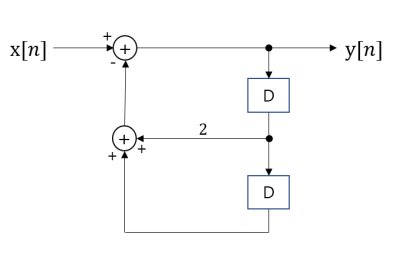
\includegraphics[width=8cm]{prob3b_probFig.png}}
\end{figure} \\
\textcolor{red}{\textbf{Solution:}}
\begin{itemize}
\item[(i)]{The difference equation which describes the system can be written as:}
\begin{equation}
\begin{gathered}
\begin{alignedat}{1}
&y[n] = x[n] -\left( 2y[n-1] + y[n-2] \right)\\
&y[n] + 2y[n-1] + y[n-2] = x[n]
\end{alignedat}
\end{gathered}
\end{equation}
\item[(ii)]{\textcolor{red}{\textbf{Homogeneous Solution:}}}
\begin{itemize}
\item[(1.)]{Let $y_{h}[n] = K z^{n}$.}
\item[(2.)]{Substituting this guess into the homogeneous difference equation will give the eigenvalues.}
\begin{equation}
\begin{gathered}
\begin{alignedat}{1}
y_{h}[n] + 2 y_{h}[n-1] + y_{h}[n-2] &=0\\
Kz^{n} + 2Kz^{n-1} + Kz^{n-2} &= 0 \\
Kz^{n-2} \left(z^{2} + 2z + 1 \right) &=0 \\
z^{2} + 2z + 1 = 0
\end{alignedat}
\end{gathered}
\end{equation}
The eigenvalues are
\begin{equation}
\begin{gathered}
\begin{alignedat}{1}
z &= \frac{-2 \pm \sqrt{2^{2} - 4(1)(1)}}{2(1)} \\
z &= -1 
\end{alignedat}
\end{gathered}
\end{equation}
\item[(3.)]{Therefore, the homogeneous solution is given by}
\begin{equation}
\boxed{y_{h}[n] = K_{h}(-1)^{n}}
\end{equation}
\end{itemize}
\item[(iii)]{\textcolor{red}{\textbf{Particular Solution:}}}
\begin{itemize}
\item[(1.)]{The input signal is $x[n] = u[n]$, which is a constant; hence, all its differences are zero. The particular solution is, therefore, also a constant}
\begin{equation}
y_{p}[n] = K_{p}.
\end{equation}
\item[(2.)]{Substituting this into the difference equation will give}
\begin{equation}
\begin{gathered}
\begin{alignedat}{1}
K_{p} + 2 K_{p} + K_{p} & = 1 \\
4K_{p} &= 1 \\
K_{p} & = \frac{1}{4}
\end{alignedat}
\end{gathered}
\end{equation}
\item[(3.)]{The particular solution is given by}
\begin{equation}
\boxed{y_{p}[h] = \frac{1}{4}}
\end{equation}
\end{itemize}
\item[(iv.)]{\textcolor{red}{\textbf{Complete Solution:}}}
\begin{equation}
\begin{gathered}
\begin{alignedat}{1}
y[n] &= y_{h}[n] + y_{p}[n] \\
y[n] &= K_{h}(-1)^{n} + \frac{1}{4}
\end{alignedat}
\end{gathered}
\end{equation}
\item[(v.)]{The system is in its zero state before $n = 0$; hence, $y[-1] = 0$ and $y[-2] = 0$. At $n=0$, therefore, $y[0] = 1$. Applying the initial condition $y[0] = 1$ gives}
\begin{equation}
\begin{gathered}
\begin{alignedat}{1}
y[0] &= K_{h}(-1)^{0} + \frac{1}{4} \\
1 &= K_{h} + \frac{1}{4} \\
K_{h} &= \frac{3}{4}
\end{alignedat}
\end{gathered}
\end{equation}
\item[(vi.)]{Therefore, the response of the system is}
\begin{equation}
\begin{gathered}
\begin{alignedat}{1}
y[n] &= 
\begin{cases}
\frac{3}{4}(-1)^{n} + \frac{1}{4}, & n \geq 0 \\
0, & n < 0
\end{cases} \\
\Aboxed{y[n] & =  \left( \frac{3}{4}(-1)^{n} + \frac{1}{4} \right) u[n]}
\end{alignedat}
\end{gathered}
\end{equation}
\end{itemize}
\end{itemize}
\end{itemize}

\pagebreak
\begin{itemize}
\item[\textbf{4.}]{\textbf{MATLAB Coding}}
\begin{itemize}
\item[\textbf{(a)}]{\textbf{Graph the function combinations with MATLAB}.}
\begin{equation}
\begin{gathered}
\begin{alignedat}{1}
x_{1}(t) &= e^{-t} \sin \left( 20 \pi t \right) + e^{-t/2} \sin \left(19 \pi t \right) \\
x_{2}(t) &= \mathtt{rect}(t) \cos \left(20 \pi t \right)
\end{alignedat}
\end{gathered}
\end{equation}

\begin{tcolorbox}[title={Source Code}]
\lstinputlisting[language=Matlab, upquote=true]{prob4a.m}
\end{tcolorbox}

\pagebreak
\begin{tcolorbox}[title={Unit-rectangle Function}]
\lstinputlisting[language=Matlab, upquote=true]{prob4a_rect.m}
\end{tcolorbox}

\begin{figure}[h!]
\center{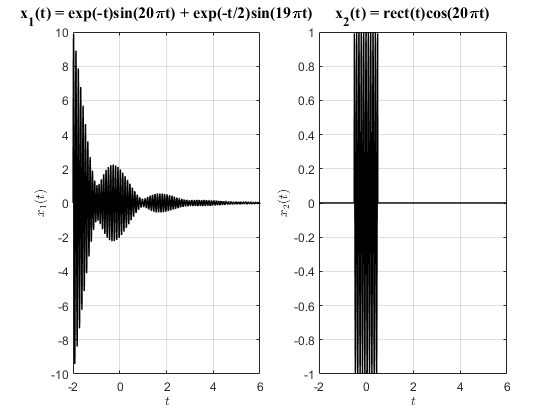
\includegraphics[width=16cm]{prob4a.png}}
\caption{\label{fig:4a}The graphs of $x_{1}(t) = e^{-t} \sin \left( 20 \pi t \right) + e^{-t/2} \sin \left(19 \pi t \right)$ and $x_{2}(t) = \mathtt{rect}(t) \cos \left(20 \pi t \right)$.}
\end{figure}

\pagebreak

\item[\textbf{(b)}]{Make sinusoid whose fundamental frequencies are the normal scale, 440 Hz (A4), 466.1 Hz (A4\#), 493.8 Hz (B4), 523.22 Hz (C5), 554.36 Hz (C5), 587.33 Hz (D5), 622.25 Hz (D5\#), 659.26 Hz (E5), 698.46 Hz (F5), 739.99 Hz (F5\#), 784.00 Hz (G5), 830.60Hz (G5\#), 880 Hz (A5).}

\begin{tcolorbox}[enforce breakable, pad at break = 1mm, break at=20cm,title={Source Code}]
\lstinputlisting[language=Matlab, upquote=true]{prob4b_Part1.m}
\end{tcolorbox}

\pagebreak
\begin{figure}[h!]
\center{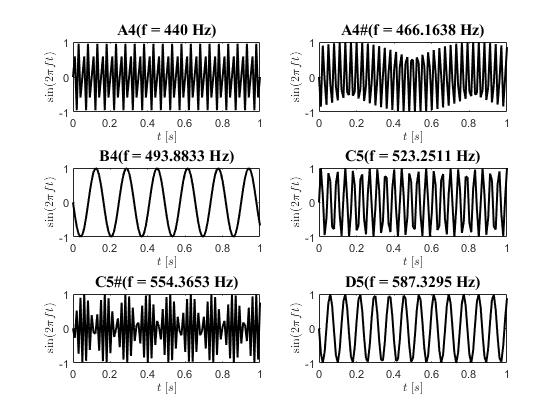
\includegraphics[width=15cm]{prob4b_graph1.png}}
\end{figure}

\begin{figure}[h!]
\center{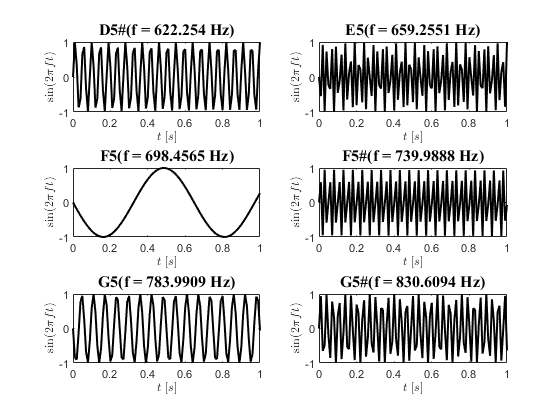
\includegraphics[width=15cm]{prob4b_graph2.png}}
\end{figure}

\pagebreak
\begin{figure}[h!]
\center{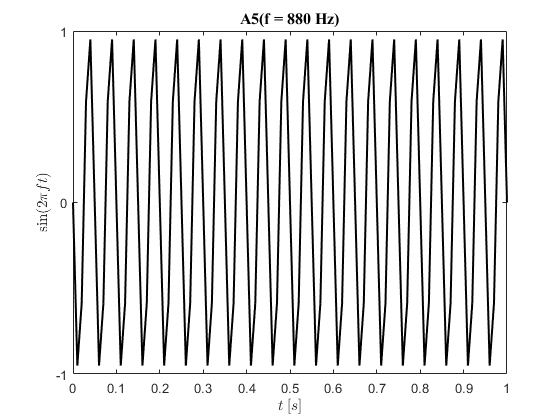
\includegraphics[width=12cm]{prob4b_graph3.png}}
\caption{Graphs of the note scales from $\mathtt{A4}$ to $\mathtt{A5}$.}
\end{figure}

\vspace{2cm}

\textcolor{red}{\textbf{Part 2:}}
Make an MP3 file containing the normal scale $\mathtt{A4}$ to $\mathtt{A5}$ one second each. \\

\begin{tcolorbox}[title={\textbf{Note:}}]
Instead of saving the file as a *.mp3 file, I have decided to just save it as a *.mp4 file because there is an $\mathtt{audiowrite()}$ function in MATLAB which can readily do this. However, *.mp3 is not supported by the  $\mathtt{audiowrite()}$.
\end{tcolorbox}

\begin{tcolorbox}[ pad at break = 1mm, break at=10cm,title={Source Code}]
\lstinputlisting[language=Matlab, upquote=true]{prob4b_Part2.m}
\end{tcolorbox}


\textcolor{red}{\textbf{Part 3:}}
Make an MP3 file containing the $/\mathtt{do}/$, $/\mathtt{re}/$, $/\mathtt{mi}/$, ..., $/\mathtt{ti}/$, $/\mathtt{do}/$. \\

\begin{tcolorbox}[title={\textbf{Note:}}]
Instead of saving the file as a *.mp3 file, I have decided to just save it as a *.mp4 file because there is an $\mathtt{audiowrite()}$ function in MATLAB which can readily do this. However, *.mp3 is not supported by the  $\mathtt{audiowrite()}$.
\end{tcolorbox}

\begin{tcolorbox}[enforce breakable, pad at break = 1mm, break at=18cm,title={Source Code: \textbf{A Major}}]
\lstinputlisting[language=Matlab, upquote=true]{prob4b_Part3_AMajor.m}
\end{tcolorbox}

\begin{tcolorbox}[enforce breakable, pad at break = 1mm, break at=15cm,title={Source Code: \textbf{A Minor}}]
\lstinputlisting[language=Matlab, upquote=true]{prob4b_Part3_AMinor.m}
\end{tcolorbox}

\vspace{2cm}
\begin{tcolorbox}[title={\textbf{Note: All the files were uploaded on GitHub}}]
All the files in this document were uploaded on Github, and can be accessed at:


\begin{center}
\url{https://github.com/rjcanoy03/BRI509/tree/Assignment%231}
\end{center}


If there are errors in the solution or codes kindly email, $\\$
recanoy@korea.ac.kr.
\end{tcolorbox}
\end{itemize}
\end{itemize}
\end{document}